\chapter{Introdução}
\label{CAP:introducao}
%\thispagestyle{empty}

Com o passar dos anos os sistemas de informação tiveram uma evolução muito grande, com essa evolução veio também um aumento significativo da quantidade de dados gerados pelos usuários, com isso os sistemas tiveram que se adaptar para poder processar essa grande quantidade de dados. 
Como exemplo da quantidade de dados gerados na rede (CANALTECH, 2012) aponta: Só o facebook gera mais de 500TB de dados por dia, de acordo com o Slash Gear, a rede social gera aproximadamente 2,7 bilhões de ‘curtir’ e 300 milhões de novas fotos são postadas no serviço diariamente, contabilizando mais de 2,5 bilhões de conteúdos processados pelo sistema no período; (TECMUNDO, 2014) mostra que cerca de 100 bilhões de buscas são realizadas no Google mensalmente; (EXAME, 2014) afirma que o conteúdo digital dobra a cada dois anos e se todo conteúdo digital do mundo fosse armazenado em ipads, eles formariam uma pilha com altura igual a dois terços da distância entre a terra e a lua. O infográfico abaixo mostra o que está acontecendo na internet a cada 60 segundos. 


\begin{figure}[htbp!] 
	\begin{center}
		% fbox faz uma borda ao redor do seu argumento		
		\fbox{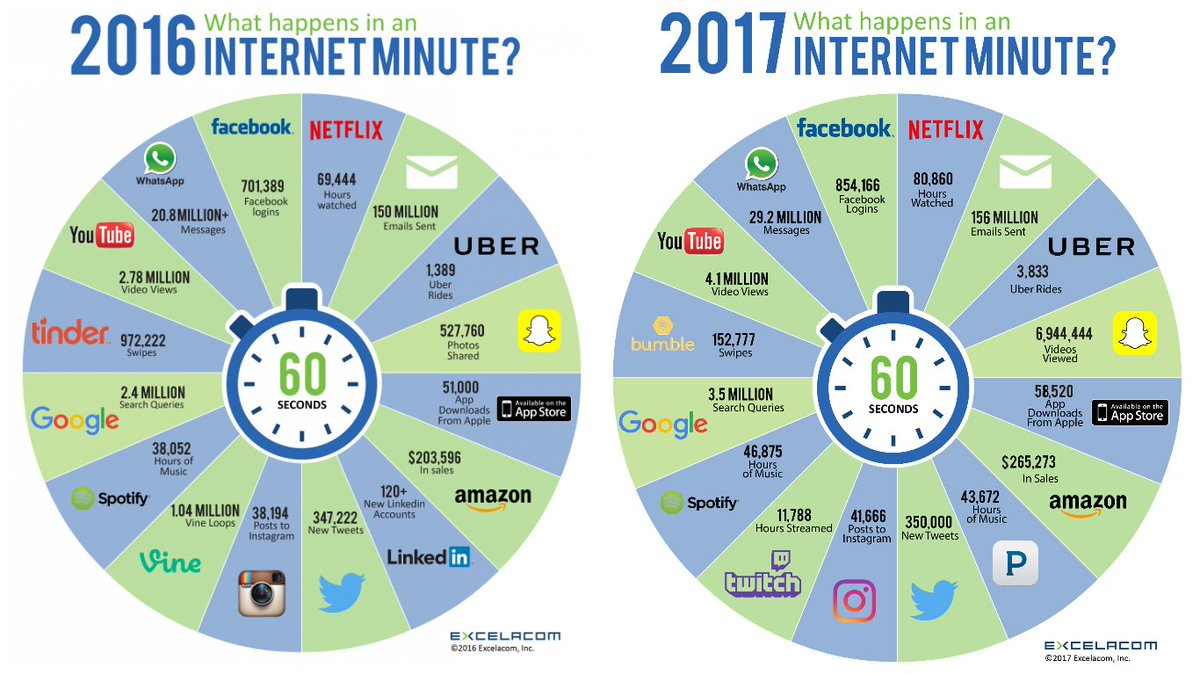
\includegraphics[width=0.80\linewidth]{figures/acontecimentoBigdata}}
		\caption{Comparação entre os anos de 2016 e 2017 do que acontece na internet a cada 60 segundos}
		\small{Fonte - (EXCELACOM, 2017)}
		\label{Fig:testeAcontecimento}
	\end{center} 
\end{figure}

Tudo isso sem contar com a IoT, onde, mais e mais dados são gerados, com sensores, leitores de RFID, smartTV, notebooks, smartphones, carros, entre outros dispositivos que geram e transmitem dados por meio da rede.

Para que a computação desta grande quantidade de informações seja realizada em tempo viável, cada vez mais faz-se necessária a exploração de paradigmas de programação paralela e processamento distribuído. Porém, desenvolver \textit{softwares} para ambientes distribuídos é uma tarefa complexa, pois envolve uma série de conceitos e problemas que devem ser considerados pelos programadores; como concorrência, tolerância a falhas, distribuição de dados e balanceamento de carga (KOLBERG, 2010).

Para armazenar e processar uma quantidade enorme de dados, foi criado o Apache Hadoop (APACHE, 2018), que é um \textit{framework} composto basicamente por dois modulos, o MapReduce para o processamento de dados de forma distribuída e o HDFS que é um sistema de arquivos escalonável e distribuído, cujo desenho é baseado fortemente no GFS (IMASTERS, 2014).

%melhorar esse parágrafo, esta muito confuso
Nas grandes empresas como Facebook, Google e Amazon, pesquisas que envolvem grandes volumes de dados, marketing direcionado, essas pesquisas são realizadas com os dados que os próprios usuários produzem. Com isso, surge alguns questionamentos. Será que os usuários sabem que seus dados estão sendo utilizados por essas empresas? Será que esses dados estão sendo armazenados de forma segura? Quais são as garantias que as empresas fornecem aos seus usuários em caso de roubo dos dados? Quais são as boas práticas de segurança utilizadas por essas empresas?

\section{Segurança em Big Data}

Nos dias de hoje, a informação passou a ser um dos bens mais preciosos das grandes organizações mundiais, não é por acaso, que os Estados Unidos espionava todos os outros paises, incluindo o Brasil, esse episódio veio a público com a revelação de um ex-técnico da CIA, conhecido como Edward Snowder em 2013 (G1, 2014).

A segurança da informação é indispensável para qualquer empresa que utiliza a tecnologia em seu dia a dia. Prevenir desastres, como perda de dados importantes ou até sofrer algum tipo de invasão de \textit{hackers}, é uma grande preocupação para os gestores (SANTOS, 2017).
Para uma boa gestão de segurança da informação é recomendado seguir em três pilares fundamentais da segurança, segundo a (NBR ISO-27002, 2013) são eles: integridade, responsável por assegurar que o conteúdo da mensagem não foi alterado, a disponibilidade, responsável por garantir que as informações estão sempre acessíveis, e a confidencialidade, responsável por assegurar o acesso à informação apenas por pessoas autorizadas.



\begin{comment}
\begin{itemize}
\item \textbf{Confidencialidade:}
A confidencialidade trata da imposição de limites de acesso à informação apenas às pessoas e/ou entidades autorizados por aqueles que detêm os direitos da informação. Ou seja, somente pessoas confiáveis podem acessar, processar e modificar os dados.\\

\item \textbf{Integridade:}
A integridade diz respeito à garantia de que as informações manipuladas conservarão todas as suas características originais. Ou seja, os dados vão se manter íntegros, conforme criados ou estabelecidos pelo proprietário.\\

\item \textbf{Disponibilidade:}
Já a disponibilidade é a garantia de que as informações estarão sempre disponíveis para o uso legítimo. Ou seja, as pessoas e/ou entidades autorizadas pelo detentor dos direitos terão sempre garantido o acesso aos dados.\\
\end{itemize}
\end{comment}

Conhecendo os pilares da segurança da informação podem-se utilizar ferramentas e mecanismos para auxiliar a segurança dos dados, dividindo-os em controle físico e controle lógico. Os controles físicos são portas, salas reservadas com seguranças, ou seja, o objetivo é proteger o ambiente físico onde encontram-se os dados, enquanto que, os controles lógicos baseiam-se em boas práticas de segurança. De acordo com (LUCENA, 2017) os controles lógicos podem ser as seguintes práticas: Criptografia, assinatura digital, honeyPot e controle de acesso.
%(Felipe Lucena SEGURANÇA DE DADOS: TUDO QUE VOCÊ PRECISA SABER 6/01/2017)

\begin{comment}
\begin{itemize}
\item \textbf{Criptografia:} Mecanismo de segurança que utiliza esquemas matemáticos e algoritmos para codificar os dados em textos inelegíveis, os quais só podem ser decodificados ou descriptografados pelas pessoas que possuem a chave de acesso.\\
\item \textbf{Assinatura digital:} Conjunto de dados criptografados, associados a um documento do qual sua função é garantir a integridade do documento, mas não a sua total confidencialidade.\\
\item \textbf{HoneyPot:} Esse é o nome dado a um software usado para detectar ou impedir ações de crackers, spammers ou qualquer outro agente externo não autorizado. Essa solução 'engana' o agente externo, fazendo-o acreditar que ele está de fato explorando uma vulnerabilidade.\\
\item \textbf{Controle de acesso:} O controle de acesso consiste em limitar o acesso a devidos usuários, de acordo com seu cargo ou conhecimento e importância dentro da organização.
\end{itemize}
\end{comment}

Existem diversas outras práticas que podem ser aplicadas nestes ambientes, como por exemplo, um \textit{firewall}, um antivírus, e entre outras técnicas específicas para ambientes diversos.

\section{Motivação}

Como explicado anteriormente, a grande quantidade de dados gerados no planeta são de extrema importância para governos e empresas, pois com os dados podem-se extrair muitas informações e com isso decisões são tomadas, sendo assim, é de suma importância que esses dados sejam protegidos de forma correta, o ambiente no qual armazena e processa os dados também deve ser protegido, com uma segurança que preveja as falhas e consiga manter os dados seguros.

Há atualmente diversas soluções tecnológicas que não habilitam quesitos mínimos de segurança durante o processo de instalação e de configuração do produto (BORDINI, 2016). Considerando que uma dessas aplicações é o Apache Hadoop, no qual a segurança não vem habilitado por \textit{default} e que há diversos tipos de riscos associados com o crescente uso de soluções de Big Data por parte das empresas, como a exposição de dados sensíveis e confidenciais na internet e o comprometimento dessas bases de dados com a exclusão, inclusão ou modificação de informações. Um estudo das vulnerabilidades de segurança no ambiente Apache Hadoop, então, pode determinar falhas de segurança e com isso boas práticas podem ser tomadas para se evitar transtornos para as empresas e usuários.

Uma maneira de estudar a segurança em Big Data utilizando o ambiente Apache Hadoop é, implementar um cenário de testes, verificar as possíveis falhas de comunicação e seu comportamento mediante ataques. Sendo assim, houve uma necessidade de montar um ambiente para que os testes pudessem ocorrer, justificando a necessidade de configurar diferentes cenários e utilizar ferramentas de invasão.

\section{Objetivos}

O Big Data, hoje em dia, mudou a forma de pensar das grandes empresas, pois as empresas detêm de muitas informações para comercializar seus produtos, como dados estatísticos, quem comprar mais, faixa etária, redes sociais, quantos cliques naquele determinado anúncio, então, isso tudo está sendo processado e está gerando infomações para que se possa lançar novas estratégias de marketing. Não só o comércio está sendo beneficiado com o grande volume de dados, o mercado financeiro, a área da saúde, e entre outras áreas.

O objetivo deste trabalho é investigar a segurança utilizada no ambiente Apache Hadoop, no qual, os dados estão armazenados e processados de forma distribuída, considerando que os dados são de extrema importância e que são valiosos, sendo assim, o trabalho propõe boas práticas de segurança para que se possa evitar perdas ou roubos de dados, tendo em vista que empresas de tecnologias importantes, tais como: MasterCard, Facebook, Google, e entre outras utilizam o ambiente Hadoop para armazenamento e processamento de grandes volumes de dados.

Além disso, este trabalho propõe analisar de forma experimental, como o ambiente Apache Hadoop se comporta durante tentativas de ataques, como por exemplo, ao executar uma tarefa pelo Apache Hadoop e tentar atacar o ambiente, como será o comportamento do \textit{framework} durante o ataque. Sabendo que a comunicação dos nós do cluster é realizada por ssh, como conseguir o usuário e a senha ou até mesmo as chaves públicas e privadas. Quais são as maneiras de burlar a segurança imposta pelo Apache Hadoop e como protegê-lo desses ataques utilizando boas práticas de segurança.

Como metodologia para atender aos objetivos deste trabalho, foram utilizadas diversas ferramentas para a criação do ambiente Apache Hadoop, tais como: o Virtual-Box, Ubuntu-Server, Kali Linux e alguns dos seus aplicativos de invasão.


\section{Metodologia}

A metodologia aplicada para a realização da análise de vulnerabilidades em ambientes Apache Hadoop é baseada na exploração de um ambiente virtualizado. A ideia principal consiste em montar um cluster e verificar suas vulnerabilidades através do sistema operacional kali linux utilizando suas ferramentas para realizar um \textit{PenTest}.

Considerado as limitações encontradas, optou-se por escolher um ambiente virtual para simular um ambiente real, tendo em vista que as maiorias dos testes são realizados antes em ambientes virtuais para que só depois possa ocorrer em um ambiente real.

Para montar o ambiente virtualizado foram utilizados \textit{softwares} gratuitos, tais como, virtual-box, ubuntu-server, kali linux e o \textit{framework} Apache Hadoop. Após montar o ambiente de teste, foram executadas algumas tarefas com o \textit{framework}, para ter a certeza de que a aplicação estava funcionando corretamente. Logo após constatar que tudo estava corretamente configurado, foi a vez de instalar e configurar o Kali linux.

Considerando que a metodologia aplicada neste trabalho é a exploração a um ambiente virtualizado, foram realizados alguns testes de invasão ao cluster, seguindo a ordem de um \textit{PenTest}, na qual obedece as etapas de reconhecimento, varredura, obtenção de acesso e obtenção das informações.

A figura \ref{Fig:EstruturaGeraldoAmbiente} apresenta a estrutura do ambiente, para uma melhor compreensão deste trabalho. Como explicado anteriormente, tanto o cluster quanto o kali linux estão na mesma rede facilitando assim a realização do \textit{PenTest}, com isso foi possível realizar ataques ao cluster.

A partir das informações da rede foi possível pensar em alguns tipos de ataque ao cluster e com isso analisar o comportamento do mesmo ao ser atacado por um usuário externo, com a utilização do \textit{software} nmap, foi possível scanear toda a rede e com isso analisar as portas abertas e as vulnerabilidades encontradas.

\begin{figure}[htbp!] 
\begin{center}
% fbox faz uma borda ao redor do seu argumento
\fbox{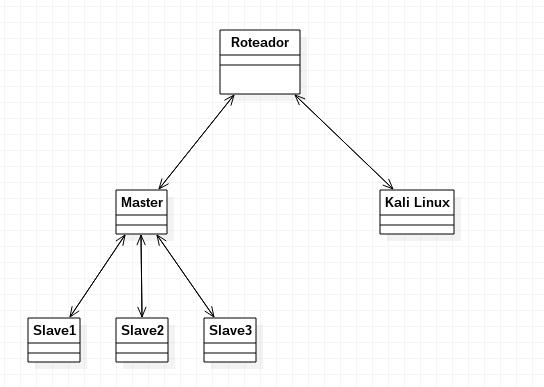
\includegraphics[width=0.80\linewidth]{figures/ClusterMelhor}}
\caption{Infográfico - Visão geral do ambiente }
\small{Fonte - (próprio autor, 2018)}
\label{Fig:EstruturaGeraldoAmbiente}
\end{center} 
\end{figure}

Pensando nas possibilidades encontradas foram sugeridos alguns ataques que poderiam levar a algum resultado significativo, os mesmos são explicados nas próximas seções.  


\subsection{Ataque de negação de serviço}
Considerando que o Apache Hadoop é um \textit{framework} resiliente a falhas, ou seja, ele saberá se comportar diante de uma falha, como por exemplo, caso um nó não funcione corretamente, os outros são capazes de suprir a necessidade, redistribuindo as tarefas para os demais nós. Então, sabendo disso, um dos ataques mais efetivos para testar isso é o ataque DoS, ou seja, apenas uma máquina atacando um nó do cluster, tentando 'derrubá-lo'.

\subsection{Ataque de força bruta}
Uma outra preocupação na utilização do \textit{framework} Apache Hadoop é que a comunicação entre os nós é realizada pelo protocolo ssh, após realizar um \textit{scanner} na rede foi possível observar que a porta 22 dos nós estavam aberta e com isso surgiu a ideia de conseguir acessar um nó através de um outro terminal remotamente.

\subsection{Ataque \textit{Man in the middle}}
Por fim, surge a ideia de realizar um \textit{man in the middle}, ou seja, ficar no meio da comunicação entre os nós, esse ataque consiste em poluir a tabela ARP da vítima induzindo ela a responder e fazer suas requisições para a máquina atacante e com isso enganá-lo.

\section{Estrutura do trabalho}

Além deste capítulo introdutório, este trabalho está organizado em mais 4 capítulos. No capítulo 2 aborda a fundamentação teórica necessária para a compreensão do trabalho. O capitulo 3 está sendo apresentado o cenário utilizado, no capitulo 4 será abordado os experimentos e resultados e o capitulo 5 a conclusão. %VOLTAR AQUI QUANDO TERMINAR O TRABALHO PARA DETERMINAR A ESTRUTURA DO TRABALHO.
